\chapter{Proposed Translator}
\label{ch:proposed-system}
As a solution to the previous chapter, this one focuses on proposing a application $f : SC' \rightarrow MO$ such that applied on a
schema, defined in \cref{eq:schema-reduction}, results in a domain model (\cref{eq:plain-object-model}) based on plain objects (\cref{eq:plain-object}).
Therefore the aim of this chapter is to once defined an schema as \cref{eq:schema-reduction} and a shape as \cref{eq:shape-reduction} define
an application $f$ such that

\begin{equation}
f(SC')=
\begin{bmatrix}f'(S'_1)
\\ f'(S'_2)
\\ \vdots
\\ f'(S'_n)
\end{bmatrix},
\end{equation}

where,

\begin{equation}
	f'(p_{SC'},t_{SC'},c_{SC'}) = (p_{S'},t_{S'}),
\end{equation}

and give a proposition for $f'(x')$ and therefore for $f(x)$.

We know that \cref{eq:shape-reduction} has been obtained in such a way that $\forall\ s' \in S'\ \exists\ f:S' \rightarrow PO$ and also in \cref{eq:values-mapping} we set
the aggregation criterion of the cardinality component over the type component to be able to create the images of $SC'$ in $MO$. Therefore $f'$ is defined as,

\begin{equation}\label{eq:transformation-f}
f':S' \rightarrow PO = f'(p_{S'},t_{S'},c_{S'}) \begin{cases}
	(p_{S'},\ Proy_{t_{S'}}lst) & if \; c_{S'}=(1,1) \\
	(p_{S'},\ List[Proy_{t_{S'}}lst]) & if \; c_{S'}=(0,\infty)
   \end{cases}
\end{equation}

where $Proy_{t_{S'}}lst$ represents the projection of the compatible type $t_{S'}$ from the shapes space of types
over the Language Specific Types space $(lst)$.

Therefore we not only know that it is possible to create a transformation from the subset of selected schemas
towards domain models formed by flat objects, but we have also identified the function that allows us to carry
out this transformation. So, next we will focus on giving shape to this function so that a system can be
implemented that performs the described transformations automatically.For this, in this section we will see
the structure of the proposed solution as well as an implementation that allows us to validate the proposed
solution to later analyze the objects generated by the solution.

\section{Structure}
Our solution is based on a code translator. In the end, a translator is still a type of compiler \cref{fig:compiler-stages},
where we have the analysis and synthesis phase. The analysis phase focuses on verifying that the input is correct and on
making the necessary transformations. While the synthesis starts from a high quality structure and performs the
appropriate transformations to reach the target representation. In the case of our solution we have a difference
and that is that we do not have a single target but multiple ones (\cref{fig:translator}).

In addition to this, in \cref{ch:proposed-sintactic-semantic-analyzer}, we have already developed a system capable of analyzing,
validating and transforming source code so that we obtained an intermediate language made up of a
high-quality graph. Therefore in our translator we will reuse the lexical, syntactic and semantic
analyzer from \cref{ch:proposed-sintactic-semantic-analyzer}, that makes the front end of our translator.
And thenm, what we will truly develop in this section, is the back-end of the translator.

\begin{figure}
    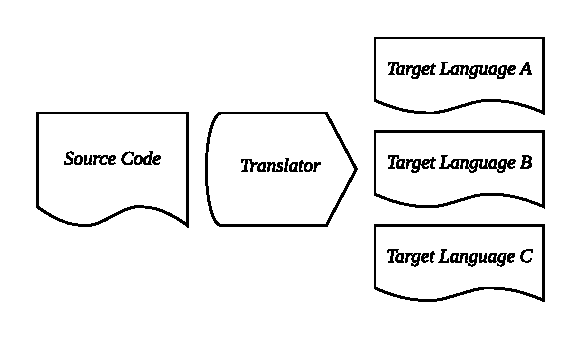
\includegraphics{images/translator.pdf}
    \centering
	\caption[Translator generic structure]{Translator generic structure.}
    \label{fig:translator}
\end{figure}

\subsection{Translator Back-end}
In our solution, the back-end of the translator, also called the synthesis phase,
fulfills two main functions. On one hand, it analyzes the intermediate language
in search of some specific incompatibility with the target language. And on the
other hand, it generates the specific code for the target language.

To perform the analysis of the intermediate language and through the Visitor pattern,
a graph path is implemented that validates that no node or set of nodes
violate the restrictions obtained in \cref{eq:schema-reduction}. The visitor that is implemented is
completely reused from the one developed for the Syntax or Semantic analysis in \cref{ch:proposed-sintactic-semantic-analyzer}.

For code generation, it is proposed to carry out an implementation of the Visitor pattern for each of the specific code generators,
each one of the specific implementations will perform the transformation function described in \cref{eq:transformation-f},
without prejudice to the fact that each specific code generator may have more implementations of the visitor associated.
\cref{fig:class-diagram-cg} illustrates this situation where the Java code generartion visitor actually contains four more visitors
one for each language specific level of the plain objects.

\begin{figure}
    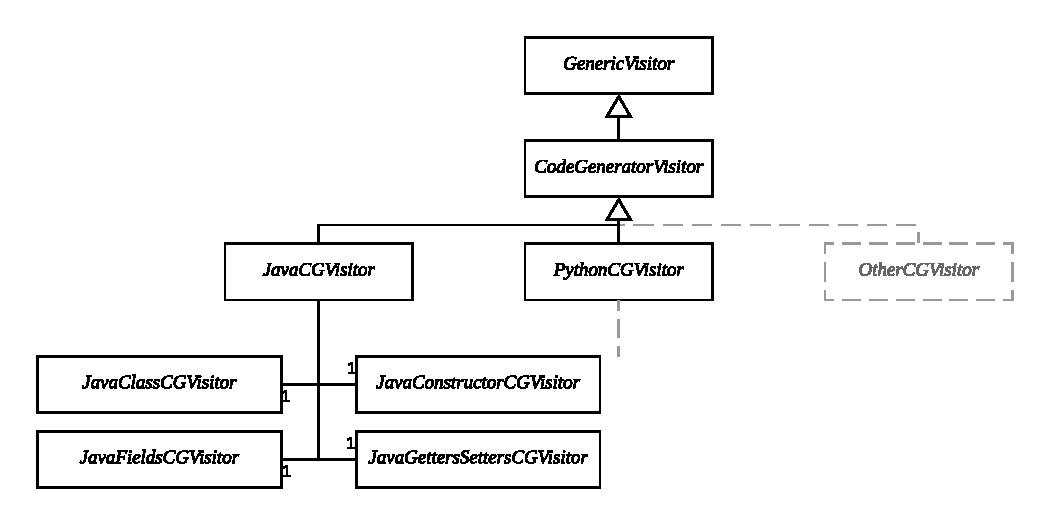
\includegraphics[width=\textwidth]{images/class-diagra-cg.pdf}
    \centering
	\caption[Class diagram example of the code generation visitors]{Class diagram example of the code generation visitors.}
    \label{fig:class-diagram-cg}
\end{figure}

\section{Implementation}

\section{Generated Obejcts}

\begin{figure}
    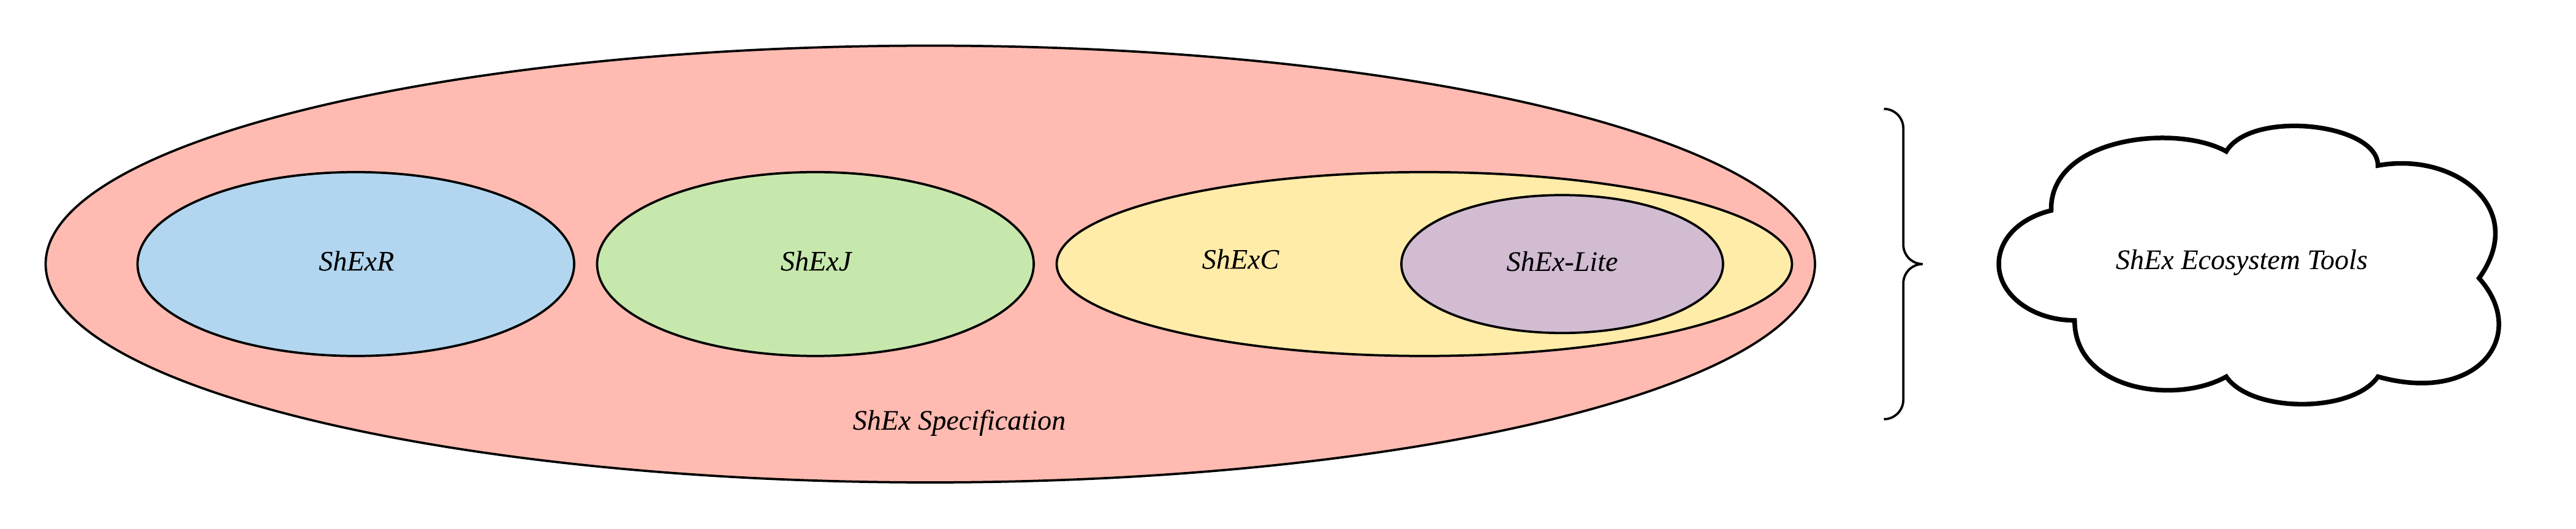
\includegraphics[width=\textwidth]{images/shex-lite-syntaxes-mental-model.png}
    \centering
    \caption[Mental model of ShEx-Lite in the existing ShEx syntaxes context.]{Mental model of
    ShEx-Lite in the existing ShEx syntaxes context. From this model we can see that Shex-Lite
    is in fact an strictly subset of ShExC, which follows the ShEx Specification. And therefore
    ShEx-Lite will also follow that expecification, which automatically enables ShEx-Lite schemas
    to be used in any other existing ShEx tool.}
    \label{fig:syntax-mental-model}
\end{figure}

\begin{figure}
  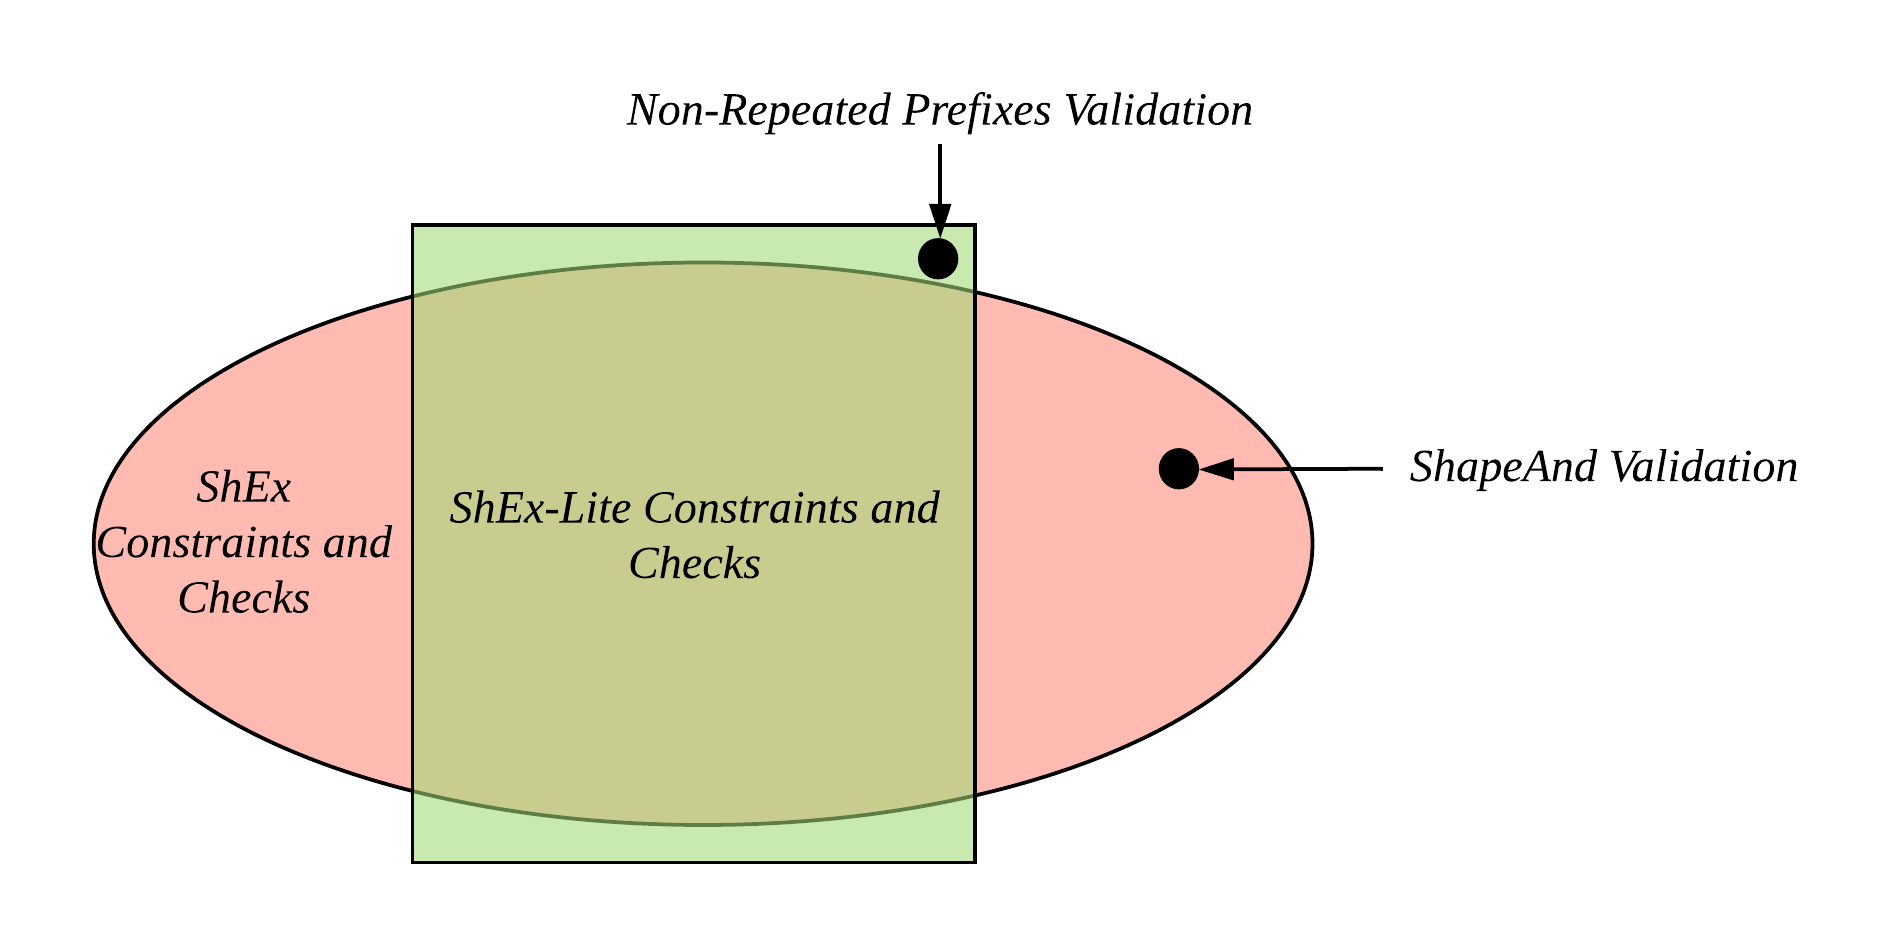
\includegraphics[width=\textwidth]{images/shex-lite-constraints-context.png}
  \centering
  \caption[Constraints and checks context diagram for ShEx-Lite and ShEx.]{Constraints
  and checks context diagram for ShEx-Lite and ShEx.}
  \label{fig:constraints-context}
\end{figure}

\begin{center}
	\noindent\begin{minipage}[t]{.4\textwidth}
		\begin{lstlisting}[frame=topline,numbers=left,title=\scriptsize\texttt{Person.shexl}, basicstyle=\ttfamily\scriptsize]{a}
# Prefixes...
:Person {
	:name xsd:string ;
	:knows @:Person *
}
		\end{lstlisting}
	\end{minipage}\hfill
	\begin{minipage}[t]{.5\textwidth}
		\begin{lstlisting}[language=Java, frame=t,numbers=left,title=\scriptsize\texttt{Person.java}, basicstyle=\ttfamily\scriptsize]{b}
// Imports...
public class Person {
	private String name;
	private List<Person> knows;
	// Constructor...
	// Getters and Setters...
}
		\end{lstlisting}
	\end{minipage}
	\captionof{figure}{Schema modeling a \texttt{Person} in \texttt{shexl} syntax to the left. And the \texttt{ShEx-Lite} generated code in \texttt{Java} to the right.}
	\label{fig:example-1}
\end{center}